%% Semantic Assistants Documentation
%% 
%% Copyright (c) 2009 Semantic Software Lab, http://www.semanticsoftware.info
%%    Rene Witte
%%    Nikolaos Papadakis
%%
\documentclass[10pt,twoside,openany,chapterprefix]{scrbook}
\usepackage{microtype}
\usepackage{bookman}
\usepackage{color}
\usepackage{url}
\usepackage{rotating}
\usepackage{listings}
\usepackage{booktabs}
\usepackage{amsmath}
\usepackage{hyperref}
\usepackage{xspace}
%\usepackage{html}
\usepackage[round, sort]{natbib}

%% package options
% KOMA-Script
\typearea{12}
%%%%%%%%%%%%%%%%%%%%%%%%%%%%%%%%%%%%%%%%%%%%%%%%%%%%%%%%%%%%
%
%  Adding lines above and below the chapter head
%
 
% 1st get a new command
\newcommand*{\ORIGchapterheadstartvskip}{}%
% 2nd save the original definition to the new command
\let\ORIGchapterheadstartvskip=\chapterheadstartvskip
% 3rd redefine the command using the saved original command
\renewcommand*{\chapterheadstartvskip}{%
  \ORIGchapterheadstartvskip
  {%
    \setlength{\parskip}{0pt}%
    \noindent\rule[.3\baselineskip]{\linewidth}{1pt}\par
  }%
}
 
% see above
\newcommand*{\ORIGchapterheadendvskip}{}%
\let\ORIGchapterheadendvskip=\chapterheadendvskip
\renewcommand*{\chapterheadendvskip}{%
  {%
    \setlength{\parskip}{0pt}%
    \noindent\rule[.3\baselineskip]{\linewidth}{1pt}\par
  }%
  \ORIGchapterheadendvskip
}
%
%  End of chapter head change
%
%%%%%%%%%%%%%%%%%%%%%%%%%%%%%%%%%%%%%%%%%%%%%%%%%%%%%%%%%%%%

%% floats
\setcounter{topnumber}{2}
\setcounter{bottomnumber}{1}
\renewcommand{\floatpagefraction}{0.9}
\renewcommand{\topfraction}{0.9}
\renewcommand{\bottomfraction}{0.9}
\renewcommand{\textfraction}{0.1}

% color definitions
\definecolor{darkred}{rgb}{0.5,0.0,0.0}
\definecolor{darkgreen}{rgb}{0.0,0.4,0.0}
\definecolor{darkblue}{rgb}{0.0,0.0,0.5}

% listing
\lstloadlanguages{Lisp,Java,Make}
\lstset{language=XML,
        basicstyle=\scriptsize\ttfamily,
        keywordstyle=\color[rgb]{0.5,0,0.33203125}\bfseries,
        frame=single,
        commentstyle=\color[rgb]{0.24609375,0.5,0.37109375}, % commentstyle=\color{blue}\ttfamily,
        extendedchars=true,
        showstringspaces=false,
        showlines=false,
        stringstyle=\color[rgb]{0.1640625,0,1}\ttfamily}
%\lstset{language=Java,basicstyle=\sffamily\footnotesize,showlines=true}

% hyperref
\hypersetup{
  backref=true,
  colorlinks=true,
  citecolor=darkgreen,
  linkcolor=darkred,
  urlcolor=darkblue,
  filecolor=red,
  letterpaper=false,
  bookmarks=true,
  bookmarksopen=true,
  pdfpagemode=UseOutlines,
  pdftitle={Semantic Assistants Documentation}, 
  pdfauthor={Semantic Software Lab}
}

%\begin{comment}
%% miscellaneous macros
\newcommand{\sfcap}[1]{\strut\vspace*{-1mm}{\footnotesize\textsf{#1}}}
\newcommand{\filetilde}{\char126$\!\!$}
\newcommand{\javadoc}[1]{\begin{tabular}{|l|}\hline
  \textbf{Visit the JavaDoc Documentation}\\
  \url{#1}\\ 
  \hline\end{tabular}}
\newcommand{\argmax}{\mathop{\mathrm{argmax}}}
\newcommand{\sa}{Semantic Assistants\xspace}

\title{Semantic Assistants\bigskip\\
\Large Guide for Users and Developers}
\author{Ren\'{e} Witte\\
Thomas Gitzinger\\
Nikolaos Papadakis\\
Bahar Sateli
\medskip}
\date{Development Release\\
\today
}
\publishers{Semantic Software Lab\\
Concordia University\\
Montr\'{e}al, Canada\\
{\large\url{http://www.semanticsoftware.info}}
}

\begin{document}
\frontmatter
\maketitle
\tableofcontents

\section*{About this document}
This document contains documentation for the \emph{Semantic
  Assistants} project. You can obtain the latest version from
\url{http://www.semanticsoftware.info/semantic-assistants}.

\section*{Acknowledgments}
The following developers contributed to the design and implementation
of the Semantic Assistants: Ren\'{e} Witte, Nikolaos Papadakis, Tom
Gitzinger.

\section*{License}
The Semantic Assistants architecture, clients, and resources are
published under the GNU Affero General Public License v3
(AGPL3)\footnote{AGPL3,
  \url{http://www.fsf.org/licensing/licenses/agpl-3.0.html}}.

\mainmatter
%% Semantic Assistants Documentation
%% 
%% This file is part of the Semantic Assistants architecture.
%%
%% Copyright (C) 2009, 2010, 2011 Semantic Software Lab, http://www.semanticsoftware.info
%%
%% The Semantic Assistants architecture is free software: you can
%% redistribute and/or modify it under the terms of the GNU Affero General
%% Public License as published by the Free Software Foundation, either
%% version 3 of the License, or (at your option) any later version.
%% 
%% This program is distributed in the hope that it will be useful,
%% but WITHOUT ANY WARRANTY; without even the implied warranty of
%% MERCHANTABILITY or FITNESS FOR A PARTICULAR PURPOSE.  See the
%% GNU Affero General Public License for more details.
%% 
%% You should have received a copy of the GNU Affero General Public License
%% along with this program.  If not, see <http://www.gnu.org/licenses/>.
%%

\chapter{Introduction to Semantic Assistants}

\section{Overview}
The \sa project aims to bring natural language processing (NLP)
techniques directly to end users by integrating them with common
desktop applications, such as word processors, email clients, or Web
browsers. To facilitate the connection between NLP frameworks and
(desktop) clients, a service-oriented architecture
(Figure~\ref{fig:arch}) has been developed that allows to integrate
(desktop) clients with NLP services implemented in the GATE
framework.\footnote{GATE, \url{http://gate.ac.uk}} NLP services are
published as standard Web services with a WSDL description.

For the general motivation, design, and background on the \sa project,
please read the information on the \sa Web site\footnote{Semantic
  Assistants,
  \url{http://www.semanticsoftware.info/semantic-assistants}} and the
contained references first \citep{giwi08,aswc08}. This document only
describes the installation and use of the developed system.

\begin{figure}[t]
  \centering
  \includegraphics[width=\textwidth]{pictures/arch}
  \caption{The \sa architecture}
  \label{fig:arch}
\end{figure}

\section{How to read this documentation}
To deploy \sa, we recommend you first read this overview chapter.
Then, consult the following parts of this documentation:

\begin{description}
\item[End Users:] Please refer to the installation guide in
  Chapter~\ref{chap:inst}, as well as the client-specific installation
  instructions in Chapter~\ref{chap:clients}. Additionally, if you
  want to run your own server, read the server installation guide
  (Chapter~\ref{chap:serv}).

\item[Language Engineers:] If you want find out how to integrate a
  GATE pipeline as a new NLP service, please refer to
  Chapter~\ref{chap:services} for documentation on the OWL service
  descriptions and Section~\ref{sec:nlpservices} for publishing the
  new service through the \sa server.

\item[Plug-in Developers:] Please first read the background material
  (Web site, papers). Then refer to the developers' notes in
  Chapter~\ref{chap:dev}.
\end{description}

\section{Architectural Overview}
\label{sec:implementation}
This section gives an overview over the current version of the Semantic
Assistants architecture, as shown in Figure~\ref{fig:arch}:

\paragraph{Tier 1} of the architecture consists of client applications
and a \emph{Client-Side Abstraction Layer (CSAL)}. Currently, there
are two example clients distributed with the system, a simple
command-line client for testing purposes and a plug-in for the
OpenOffice.org \emph{Writer} word processor. The client-side abstraction
layer consists partly of hand-written Java classes that provide
common client-side functionality, partly of automatically generated
Java classes. The communication between client and server is
implemented by means of W3C Web services.\footnote{Web Services Architecture, see
  \url{http://www.w3.org/TR/ws-arch/}} 

\paragraph{Tier 2} of the architecture consists of a \emph{Web server}
and the \emph{NLP Service Connector}. The Web server used by default
in the architecture is the Java~6 embedded Web server.  The NLP
Service Connector currently integrates the GATE framework for NLP. It
is responsible for a number of tasks, including communication with the
client, reading and querying the language service descriptions,
running requested language services, and generating response messages.

\paragraph{Tier 3} is the NLP subsystem. At present, only the GATE
framework is supported (future work might integrate additional
frameworks, such as UIMA).  It makes use of the GATE API in order to
assemble language services, store them in a permanent way, and invoke
them when they are requested by a client.

\paragraph{Tier 4} is the resource tier.  Here we have the language
service descriptions, which are authored in the Web Ontology Language
(OWL).  Tier~4 further contains external documents, which the NLP
subsystem must be able to access. Finally, we possibly have
pre-indexed documents as part of the resources tier. For indexing,
GATE uses Apache's Lucene indexer\footnote{Apache Lucene, see
  \url{http://lucene.apache.org/}} as a subsystem, and allows us,
through its API, to create and access indices.


\section{System Components}
\label{sec:syscomp}
The implementation of the Semantic Assistants architecture currently comes
with the following components:

\begin{description}
\item[Server:] The server is the core of the architecture.  It
  communicates with the clients through the CSAL on one hand and
  the NLP framework through the NLP Service Connector on the other.
  At present, the architecture only contains a connector for
  GATE. However, it was explicitly designed to allow an easy
  integration of other frameworks (for example, UIMA). For describing
  available services, we use ontology-based (OWL) service
  descriptions. As a service-oriented architecture (SOA), every
  service is automatically available to all clients connected to the
  architecture, using standard WSDL\footnote{Web Services Description
    Language (WSDL), see \url{http://www.w3.org/TR/wsdl}}) interface
  descriptions.

\item[Client-Side Abstraction Layer (CSAL):] Our top goal was to make
  it as easy as possible for client (plug-in) developers to integrate
  NLP functionality. As clients should be able to connect to the
  architecture entirely by ``local'' means, we provide an
  \emph{abstraction layer}, named CSAL, which is located on the client
  side and performs the actual communication with the server.

  Apart from the communication functionality, the CSAL also provides
  common client-side functionality, i.e., useful data types and
  methods that are frequently required when integrating NLP into
  desktop clients.

\item[Clients:] Two example clients come with the architecture: a
  command-line client and a plug-in for the OpenOffice.org Writer word
  processor. 

\item[Example Resources:] NLP functionality is provided to clients
  through Web services. To match clients with suitable services
  (depending on language, formats, etc.), each NLP service comes with
  a semantic service description in OWL format. Three example service
  descriptions are included in the current distribution: an
  information extraction (IE) service that detects persons and locations
  (using GATE's ANNIE pipeline), an IR service (using the Yahoo PR)
  and a compound service, which combines the IR and the IE
  service. These should help you in defining your own NLP services
  that you deliver to your end users (e.g., summarization,
  question-answering, domain-specific NLP services).

\item[Documentation and Online Resources:] Apart from this guide, a
  number of publications on the \sa are available
  online,\footnote{\sa,
    \url{http://www.semanticsoftware.info/semantic-assistants}} as
  well as a discussion forum for support.
\end{description}


% \begin{figure}
%   \centering
%   %\vspace*{-9mm}
%   \includegraphics[width=0.6\textwidth]{pictures/abstraction.jpg}
%   \caption{We introduce a client-side abstraction layer}
%   \label{fig:abstraction}
%   %\vspace*{-0.4cm}
% \end{figure}

\section{Example NLP Services}
A number of example pipelines (NLP services) come with the architecture.
They are located in the \url{Resources} directory. There are two
parts: the semantic service descriptions in OWL format stored in the
\url{OwlServiceDescriptions} directory and corresponding GATE
pipelines (\url{.xgapp} files) implementing these services in the
\url{GatePipelines} directory.

\paragraph{Person and Location Extractor.} This NLP service runs the
ANNIE IE system that comes with the standard GATE distribution.  It
detects a number of named entities, such as persons, locations,
organizations, etc.  An OWL service description for this pipeline is
already implemented and stored in the directory
\url{Resources/OwlServiceDescriptions/annie.owl}.  For details on the
OWL-based description format, please refer to Section~\ref{sec:owl}.

\paragraph{Yahoo Search.} This service performs a Web search for a
user and returns the first $n$ documents (where $n$ is a
user-configurable runtime parameter). While this service usually works
as provided, you should obtain a Yahoo API key (see the
\href{http://gate.ac.uk/sale/tao/splitch19.html#x24-51700019.7}{GATE
  manual} for details on this) and store this key in the file
\url{Resources/GatePipelines/Yahoo/application.xgapp} by replacing the
string ``insertyahooidhere'':
\begin{verbatim}
    <string>applicationID</string>
    <string>insertyahooidhere</string>
\end{verbatim}

\paragraph{Web IR Extractor.} The third example service shows how to
combine two existing services, by first calling the Yahoo IR service
and then using the search results as input to the ANNIE IE
service. This service is located in \url{yahooExtractor.owl}.

\section{Service Output Types}
Following a successful execution of an NLP service, the generated results are sent to the clients in form of an XML document. Each result can have one of the following types:

\paragraph{Annotation} Annotation results are extracted entities that bear a \texttt{start} and \texttt{end} offset that represent the location of the annotation in their source document's text. Annotation instances are often highlighted in the text using their offsets or presented to users in lists, based on their implementation in various clients. In addition to offsets, annotation instances has \texttt{content} and \texttt{type} attributes that holds the annotation's textual content, i.e., the text between the two offsets, and their type. For example. the Person and Location Extractor service generates annotation instances of ``Person'' and ``Location'' types. Furthermore, Annotations hold additional information if they are provided with so-called \texttt{features}. Features are an unlimited list of additional information associated to an annotation in form of key and value pairs. For example, an annotation of type Person can have a \texttt{Gender} feature.
\paragraph{Boundless Annotation} Boundless annotations are special kind of annotations that adhere to the whole document and have no start and end offsets. Like Annotation instances, they may hold a list of features. The handling behaviour of such annotations are dependent of the clients implementations.  
\paragraph{File} Files generated by NLP services are stored on the server running the service and their identifiers along with some format information are merely passed to clients. Each file result has a \texttt{url}, a \texttt{mimeType} and \texttt{format} attribute representing a human-readable description of its mime type. The client can evaluate this information, and, if it decides to do so, request the result  file itself by using the identifier sent to it. The server then sends the actual file and it is up to the client implementation on how to present it,


% Semantic Assistants - http://www.semanticsoftware.info/semantic-assistants

% This file is part of the Semantic Assistants architecture.

% Copyright (C) 2009, 2010, 2011 Semantic Software Lab, http://www.semanticsoftware.info
% The Semantic Assistants architecture is free software: you can
% redistribute and/or modify it under the terms of the GNU Affero General
% Public License as published by the Free Software Foundation, either
% version 3 of the License, or (at your option) any later version.
   
% This program is distributed in the hope that it will be useful,
% but WITHOUT ANY WARRANTY; without even the implied warranty of
% MERCHANTABILITY or FITNESS FOR A PARTICULAR PURPOSE.  See the
% GNU Affero General Public License for more details.
 
% You should have received a copy of the GNU Affero General Public License
% along with this program.  If not, see <http://www.gnu.org/licenses/>.

\chapter{Installation}
\label{chap:inst}
\emph{Note: at present, the installation has been tested under
  Linux and Mac OS X}

\section{Download}
To download the latest version of the \sa and this documentation
please refer to
\url{http://www.semanticsoftware.info/semantic-assistants-architecture}.
A pre-compiled build of the latest version is available from our
Hudson server, \url{http://assistant.cs.concordia.ca:8080/}. In the
following, we assume you use a pre-compiled version; for compilation
instructions, please refer to Chapter~\ref{chap:dev}.

\section{Prerequisites}
To deploy the \sa architecture, a number of other (open source)
components are needed:

\paragraph{Common throughout the Project:}
\begin{enumerate}
%  \item  Apache ANT, \url{http://ant.apache.org/}
  \item  Sun JDK 6, \url{http://java.sun.com/javase/downloads/index.jsp}
  \item  GATE v6.0 or newer, \url{http://gate.ac.uk/}
\end{enumerate} 

\paragraph{For the \sa Server:}
\begin{enumerate}
  \item Java API for XML Web Services (JAX-WS) v2.1.x, \url{https://jax-ws.dev.java.net/}
%  \item Prot\'{e}g\'{e}-OWL API v3.4, \url{http://protege.stanford.edu/plugins/owl/api/} 
\end{enumerate}

\paragraph{For the CSAL:}
\begin{enumerate}
  \item Java API for XML Web Services (JAX-WS) v2.1.x, \url{https://jax-ws.dev.java.net/}
\end{enumerate}

\paragraph{For the OpenOffice.org Writer Plug-in:}
\begin{enumerate}
\item OpenOffice 3.2, \url{http://download.openoffice.org/}
\item The OpenOffice.org 3.2 SDK,
  \url{http://download.openoffice.org/sdk/index.html}
%\item Apache log4j v1.2,
%  \url{http://logging.apache.org/log4j/1.2/index.html}
%\item Apache Commons Lang v2.4, \url{http://commons.apache.org/lang/}
\end{enumerate}

\paragraph{For the Eclipse Plug-in:}
\begin{enumerate}
\item Eclipse Classic 3.5+ \url{http://www.eclipse.org/downloads/}
\end{enumerate}


\section{Path Configuration}
\label{sec:props}
The \emph{SemassistProperties.xml} file serves for two purposes.  It's
included by the ANT \emph{build.xml} files of all projects and
contains common directory paths and used to compile the various
Semantic Assistants components. Secondly, it used by the server at
run-time as a property file.

Users needs to modify the values of the properties in order to
correspond at the proper paths of their machine. The options to be
adapted, include the path to the service description directory, GATE
home, GATE plug-ins, etc. Descriptions of these properties are as the
followings:

The first part is an import statement, where it includes the
\texttt{LocalProperties.xml} file. This file the is the place to store
your local paths and customizations, e.g., you can add additional paths
for your local pipelines in this file.
\begin{lstlisting}[language=XML,numbers=left,xleftmargin=8mm,columns=flexible]
    <!-- Importing LocalProperties.xml file for local paths and customizations -->
    <import file ="LocalProperties.xml"/>
\end{lstlisting}
By default, \texttt{LocalProperties.xml} contains the path to the directory containing the NLP
service descriptions (OWL files):
\begin{lstlisting}[language=XML,numbers=left,xleftmargin=8mm,columns=flexible]
  <property name="service.repository"       value="${semassist.home}/Resources/OwlServiceDescriptions/"/>

  <path id="localruntimeclasspath">
    <!-- Added locally needed paths here -->
  </path>
\end{lstlisting}


The second part of the \texttt{SemassistProperties.xml} is where the
machine-specific variables are modified to point to proper paths of
the users' machine. The variables as follows:
\begin{lstlisting}[language=XML,numbers=left,xleftmargin=8mm,columns=flexible]
    <!-- Machine dependent properties.Need to be modified -->
    <property name="durmtools"          value="/usr/local/durmtools" />
    <property name="jaxws.home"         value="${durmtools}/jaxws-ri" />
    <property name="gate-home"          value="${durmtools}/GATE/gate" />
    <property name="jdk.home"           value="${durmtools}/jdk" />
\end{lstlisting}

\begin{enumerate}
\item \url{durmtools}: This is one of the most important variables in this properties file and needs to be defined properly. According to the prerequisites mentioned earlier, there are various applications that need to be installed prior to using the Semantic Assistants.
Create a folder called \texttt{durmtools} and install all the required applications to this folder, or point this variable to where all your applications are installed e.g. \emph{Applications} on Mac or \emph{Programs} in Windows.
%\item \url{semassist.home}: This variable points to the place on your local machine that the Semantic Assistants package has been downloaded and extracted. Put the full path of the folder in here, exempting the user home directory path for it will be automatically replaced by \texttt{\$\{user.home\}}.
%\item \url{csal.home}: This variable points to the \texttt{CSAL} folder inside the Semantic Assistants package. If the structure is untouched, the path should read \texttt{"\$\{semassist.home\}/CSAL"}.
\item \url{jaxws.home}: This variable points to the Java API for XML Web Services (JAX-WS) v2.1.x application installed in the path defined in \texttt{\$\{durmtools\}} variable.
%\item \url{protege-home}: This variable points to the Prot\'{e}g\'{e}-OWL API v3.4 application installed in the path defined in \texttt{\$\{durmtools\}} variable.
\item \url{gate-home}: This variable points to the GATE v6.0 or newer application installed in the path defined in \texttt{\$\{durmtools\}} variable.
\item \url{jdk.home}: This variable points to the Sun JDK 6 installed on your machine.
\end{enumerate}


The third part includes all the properties used by the OpenOffice.org Writer plug-in. Therefore, in order to use this plug-in, all these variables should be defined beforehand.
\begin{lstlisting}[language=XML,numbers=left,xleftmargin=8mm,columns=flexible]
    <!-- Used by Open Office Writer Plug-In-->    
    <property name="office.home.dir"          value="${durmtools}/OpenOffice"/>
    <property name="uno-copy-dest"  	      value="${user.home}/Documents/uno-components" />
    <property name="office.program.dir"       value="${office.home.dir}/program"/>
    <property name="ooo-classes-basis"        value="${office.home.dir}/basis3.2/program/classes/" />
    <property name="ooo-classes-common"       value="${office.home.dir}/ure/share/java/" />
\end{lstlisting}
\begin{enumerate}
\item \url{office.home.dir}: This variable points to the OpenOffice 3.2 application installed in the path defined in \texttt{\$\{durmtools\}} variable explained earlier.
\item \url{uno-copy-dest}: This variable identifies where the Semantic Assistants plug-in will be stored when it is successfully built. 
\item \url{office.program.dir}: This variable points to the \texttt{program} folder inside \texttt{\$\{office.home.dir\}} path which contains the Writer program.
\item \url{ooo-classes-basis}: This variable points to the folder that contains the bulk, brand-independent OpenOffice functionalities.
\item \url{ooo-classes-common}: This variable points to the folder that containes common Java JAR libraries used by OpenOffice.
\end{enumerate}

The next part includes all the properties used by the Eclipse plug-in. Therefore, in order to use this plug-in, all these variables should be defined beforehand.
\begin{lstlisting}[language=XML,numbers=left,xleftmargin=8mm,columns=flexible]
    <!-- Used by Eclipse Plug-In-->
    <property name="eclipse.program.dir"      value="${durmtools}/eclipse-4.0"/>
    <property name="eclipse.plugins"          value="${eclipse.program.dir}/plugins"/>
\end{lstlisting}
\begin{enumerate}
\item \url{eclipse.program.dir}: This variable points to the Eclipse v3.5 or newer application installed in the path defined in \texttt{\$\{durmtools\}} variable explained earlier.
\item \url{eclipse.plugins}: This variable points to the \texttt{plugins} folder located inside the Eclipse application installed on your machine.
\end{enumerate}

The last part includes all the properties used by the Semantic Assistants server at runtime.
\begin{lstlisting}[language=XML,numbers=left,xleftmargin=8mm,columns=flexible]
    <!-- Used by the server at runtime as properties -->
    <property name="gate.plugin.dir"          value="${gate-home}/plugins/"/>
    <property name="gate.user.file"           value="${semassist.home}/Server/gate-home/user-gate.xml" />
    <property name="ontology.repository"      value="${semassist.home}/Resources/ont-repository/" />

    <property name="runtime.maxmem"       value="1638m" />
    <property name="runtime.heap.initial" value="128m" />
    <property name="runtime.heap.max"     value="1638m" />
    
    <!-- Server Property Settings (ie # of Threads allowed) -->
    <property name="server.threads.allowed"        value="3"/>

    <!-- Port for which the Server listens for debugers to be attached -->
    <property name="server.port.debug"    value="8885"/>
    
    <!-- Port used by the Server to communicate with the clients through wsdl-->
    <property name="server.port.wsdl"     value="8879"/>
\end{lstlisting}
\begin{enumerate}
\item \url{gate.plugin.dir}: This variable points to the GATE application \texttt{plugins} folder used for service executions.
\item \url{gate.user.file}: This variable points to the GATE application user configuration file.
%\item \url{service.repository}: This variable points to the OWL service description files. New service description files are added to this folder once they're available and will be later detected by the server. 
\item \url{ontology.repository}: This variable points to the folder containing the SemanticAssistants OWL files.
\item \url{runtime.maxmem}: This variable contains the maximum amount of runtime memory used by JDK. Unless your JDK complains about the value, leave this as it is.
\item \url{runtime.heap.initial}: This variable contains the initial amount of heap space used by JDK at runtime.
\item \url{runtime.heap.max}: This variable contains the maximum amount of heap space used by JDK at runtime.
\item \url{server.threads.allowed}: This variable contains the number of threads the server should allow to run concurrently.
\item \url{server.port.debug}: This variable contains the port number on users machine on which the server listens for debuggers to be attached.
\item \url{server.port.wsdl}: This variable contains the port number on which the server communicates with the clients through WSDL.
\end{enumerate}


\section{Client Installation}
The installation and configuration of clients is covered in
Chapter~\ref{chap:clients}.

\begin{description}
\item[Command-Line Client:] For information on how to compile and run
  the command-line client, please refer to Section~\ref{sec:sacl:clc}.

\item[The OpenOffice.org Writer Plug-In:] For details on how to
  compile and run the OpenOffice.org Writer plug-in please refer to
  Section~\ref{subsec:oo-inst}.

\item[The Eclipse Plug-In:] For details on how to
  compile and run the Eclipse plug-in please refer to
  Section~\ref{subsec:eclipse_install}.
\end{description}










%% Semantic Assistants Documentation
%% 
%% This file is part of the Semantic Assistants architecture.
%%
%% Copyright (C) 2009, 2010, 2011 Semantic Software Lab, http://www.semanticsoftware.info
%%
%% The Semantic Assistants architecture is free software: you can
%% redistribute and/or modify it under the terms of the GNU Affero General
%% Public License as published by the Free Software Foundation, either
%% version 3 of the License, or (at your option) any later version.
%% 
%% This program is distributed in the hope that it will be useful,
%% but WITHOUT ANY WARRANTY; without even the implied warranty of
%% MERCHANTABILITY or FITNESS FOR A PARTICULAR PURPOSE.  See the
%% GNU Affero General Public License for more details.
%% 
%% You should have received a copy of the GNU Affero General Public License
%% along with this program.  If not, see <http://www.gnu.org/licenses/>.
%%

\chapter{The \sa Server}
\label{chap:serv}
Semantic NLP services are executed by a Semantic Assistants
server. You can either use an existing server (e.g., from your
company's or university's intranet, or a public server) or run you own
server locally. To access to an existing server, you need to know it's
hostname and port, which are then configured in the client plug-ins
through a preference window.  If you want to run your own server using
the included example NLP services, follow the instructions below.

\section{Starting the Server}
Type \texttt{ant run} in the \url{SemanticAssistants/Server} directory
to start the server. Please refer to Section~\ref{sec:inst-comp} for
more installation and compilation details. The server will
automatically load all available OWL service descriptions from the
default location \url{Resources/OwlServiceDescriptions} and publish
these to the clients.

\subsection{Configuring the Server User Request Limit}
To configure the server to limit the amount of user requests it will
process concurrently, one needs to modify the \texttt{server.thread.allowed}
found in \url{SemanticAssistants/SemassistProperties.xml};  The default
value is already set but if ommitted the number of threads that will
be allowed will not necessarily reflect the server capabilities.

\subsection{Configuring the Server Fixed Pipelines}
The server comes with the possibility to set the number of concurrent threads
of the same pipeline (see GATE documentation for pipeline definition).  To 
configure these settings, one must modfiy/add the following lines
\begin{enumerate}
\item \texttt{server.pipeline.\#.name}
\item \texttt{server.pipeline.\#.number.pooled}
\item \texttt{server.pipeline.\#.max.concurrent}
\item \texttt{server.pipeline.\#.startup}
\item \texttt{server.pipeline.\#.fullpath}
\end{enumerate}
(**note: the '\#' must be replaced by a valid positive integer value)
These lines refer to the pipeline that will be pooled for concurrent and
speedier access.  
``name'' refers to the name of the pipeline as indicated by the contents of the .xgapp file.
``number.pooled'' refers to the number of threads we have allocated for this pipeline.
``max.concurrent'' refers to how many threads you will allow to run concurrently.  This number is not permanent as the pipeline completes the numbers will return to the ``number.pooled'' value
``startup'' indicated by a "true"/"false" string value which loads or ignores the pipeline at server startup.
``fullpath'' refers to the location of the xgapp file that will be used to load the pipeline.
These properties must be grouped and must be a set when being used in the \url{SemanticAssistants/SemassistProperties.xml};
These properties can be omitted if desired and only the \texttt{server.thread.allowed} will be taken into account
One must be aware that the number of pipelines set in \texttt{server.pipeline.\#.number.pooled}
will be substracted from the \texttt{server.thread.allowed} property.  Should the number previously
set in \texttt{server.thread.allowed} not be sufficient, the server will automatically resize the property
to contain the total number of threads needed.

\subsection{Testing the Server by accessing the WSDL}
To test if the Server is operating open your favourite browser and
paste \url{http://<server host>:<server port>/SemAssist?wsdl} (Note
the \texttt{<server host>} has a default value of the local machine
name and the \texttt{<server port>} is the value of the property
\texttt{server.port.wsdl} found in
\url{SemanticAssistants/SemassistProperties.xml}; by default it is set
to 8879.

On most platforms, either \url{http://localhost:8879/SemAssist?wsdl}
or \url{http://127.0.0.1:8879/SemAssist?wsdl} should show you the WSDL
if the server has been initialized correctly.\footnote{If this does
  not work, try substituting the current IP address for
  localhost/127.0.0.1 and check that the port is not blocked by a
  firewall.}

\subsection{Server Testing using the Command Line Client}
To test if the server is running correctly and can be accessed from
the clients, we recommend you run some tests using the command-line
client described in Section~\ref{sec:sacl:clc}.


\section{Integrating New NLP Services}
\label{sec:nlpservices}
For the server to know how to handle the different NLP services
offered through the architecture, it needs a \emph{description} of
each offered service. These are by default located in the
\url{SemanticAssistants/Resources/OwlServiceDescriptions}
directory. The GATE pipelines corresponding to these service
descriptions are located (by default) in
\url{Resources/GatePipelines}. The language service descriptions are
ontologies, building on the \emph{SemanticAssistants.owl} ontology,
which, in turn, extends the \emph{ConceptUpper.owl} ontology. Both of
these are located in \url{ont-repository} under
\url{SemanticAssistants/Resources}.

The details for developing new NLP service descriptions are covered in
Chapter~\ref{chap:services}.  In order to create a new language
service description, it is often easier to copy an old one and edit
it. Prot\'{e}g\'{e}\footnote{Prot\'{e}g\'{e},
  \url{http://protege.stanford.edu}} is helpful as an ontology
editor. Most important is to define the parameters that can be passed
to this language service, as well as the description of the results
that should be passed back to the client.

In summary, to integrate a new NLP service, two steps are necessary:
\begin{enumerate}
\item Store the GATE pipeline implementing the service under
  \url{Resources/GatePipelines} (using GATE's \emph{Save Application State}
  or \emph{Export to Teamware} menu functions).
\item Develop an OWL service description for this pipeline.  For
  details on the OWL NLP description format, please refer to
  Section~\ref{sec:owl}.
\end{enumerate}

\section{\sa RESTful Interface} In addition to the SOAP interface described above, the \sa server also offers a RESTful interface. This server interface conforms to the REpresentational Transfer Protocol\footnote{REST Web Architecture, \url{http://dl.acm.org/citation.cfm?doid=514183.514185}} constraints and allows clients to inquire and invoke NLP services via light-weight HTTP requests. The current supported actions of our RESTful interface are \texttt{GET} and \texttt{POST} requests and its default representation format is XML. Table~\ref{tab:rest_actions} shows the how to use the \sa RESTful web interface.

\begin{table}[htb]
 \centering\small\sffamily
 \begin{tabular}{p{0.25\textwidth}@{\hspace*{4mm}}p{0.07\textwidth}@{\hspace*{4mm}}p{0.6\textwidth}}
   \toprule
   \textbf{URL} & \textbf{Method} & \textbf{Application} \\
   \midrule
   /services & GET &
   \emph{Retrieves the representation of all available assistants} \\

   & & \\

   /service/\{serviceName\} & POST & \emph{Invokes the specified service} \\

   & & \\
   
   /users & GET & \emph{Retrieves the representation of all users (requires admin access)} \\
   
      & & \\

   /user/\{username\} & POST & \emph{Registers a new user} \\

& & \\

   /user/\{usename\} & GET & \emph{Retrieves the representation of the specified user} \\

   \bottomrule
\end{tabular}
 \caption{The \sa RESTful Web Interface}
 \label{tab:rest_actions}
\end{table}
 
 \subsection{Deployment Options}
 The \sa RESTful web interface is essentially a Java Web Archive (WAR) file that like any other Java web application, needs be deployed in a web container. In the following, we describe how the \sa WAR file can be automatically deployed on an Apache Tomcat\footnote{Apache Tomcat Web Server, \url{http://tomcat.apache.org/}} server as well as inside a console.
 
Before proceeding to deploy the server, we have to build the WAR file first. To do so, browse to \url{SemanticAssistants/Server-REST} folder and type \texttt{ant pack}. This command will automatically resolve all the dependencies of the RESTful project, compiles the source code and builds a WAR file, named  \texttt{SemAssistRestlet.war}, in the \url{dist} folder.
 
\subsubsection{Deploying on Apache Tomcat}
Apache Tomcat is an open source web server and a container for Java web applications. The Ant build script in the \url{Server-REST} folder has a special target that automatically deploys the \url{SemAssistRestlet.war} file on a provided Tomcat installation file using the Tomcat's Manager application. The Manager application allows deploying and undeploying various applications without the need to restart the Tomcat server.

To use this option, you need:

\begin{itemize}
\item A Tomcat installation on your system
\item The Tomcat Manager application\footnote{The Manager application is installed by default on context path \texttt{/manager} in Tomcat 5 and later.}
\item Have Tomcat and Manager user credentials in hand\footnote{You can find these credentials in \texttt{\$TOMCAT\_HOME/conf/tomcat-users.xml} file.}
\end{itemize}

Once you have the Tomcat and Manager credentials, proceed to edit the \texttt{build.xml} file in \url{SemanticAssistants/Server-REST} folder. Find the following lines in the file and replace the dummy values with your credentials:

\begin{lstlisting}[language=XML,numbers=left,xleftmargin=8mm,columns=flexible]
    <!-- tomcat properties - replace with correct values -->
    <property name="tomcat.manager.url"       value="http://localhost:8080/manager"/>
    <property name="tomcat.manager.username"       value="test"/>
    <property name="tomcat.manager.password"       value="test"/>
\end{lstlisting}

Now type \texttt{ant deploy} in your console for the Ant script to automatically deploy the \url{SemAssistRestlet.war} file in your Tomcat. You can test the RESTful interface by pointing your browser to \texttt{http://localhost:8080/SemAssistRestlet/services}. If the application is successfully deployed in Tomcat, you should see an XML document listing available services of the connected \sa server.

Similarly, you can stop or undeploy the RESTful interface using \texttt{ant stop} and \texttt{ant undeploy} commands respectively.
 
\subsubsection{Running as a standalone application}
The \url{SemAssistRestlet.war} file comes with an embedded Jetty\footnote{Jetty Web Server, \url{http://jetty.codehaus.org/jetty/}} web server that allows the application to run without the need for an external web container. Embedding the Jetty server inside our application, creates an executable WAR file that requires nothing but a Java runtime environment to run. In order to start the RESTful server, browse to \url{SemanticAssistants/Server-REST/dist} and type \texttt{java -jar SemAssistRestlet.war}. This command will start the RESTful web server on its default port \texttt{8182} and print logs on your console. To test the server, open your web browser and go to \texttt{http://localhost:8182/services}. If the server has started successfully, you should see an XML document in your browser that presents a list all the available services in the connected \sa server.

You can also run the RESTful server on a custom port. To do this, send your preferred port number as an input argument to the executable WAR file by typing \texttt{java -jar SemAssistRestlet.war 1234}. This command will start the server on \texttt{http://localhost:1234}.

\section{Server Authentication}
One of the major concerns when transmitting data in a client-server architecture is the protection of data from being sniffed or hijacked by eavesdroppers. This can be achieved by encrypting the communication channel with cryptographic algorithms. HyperText Transfer Protocol Secure (HTTPS) is a combination of HTTP and Secure Socket Layer (SSL) protocol that uses industry-strength encryption algorithms to secure a channel between a client and a server. In addition, it allows clients to verify the authenticity of the server that they are sending their data to. The \sa RESTful web server also offers a secure interface that is published on the HTTPS protocol. 

To start the secure interface, browse to the \url{SemanticAssistants/Server-REST/dist} folder and type \texttt{java -jar SemAssistRestlet-Secure.war}. Then point your web browser to \texttt{https://localhost:8183/services}. Your browser should prompt you saying that the certificate of this URL is not verified. This is because the certificate that the RESTful web server is presenting to your browser is not verified by a leading SSL Certificate Authority, since it is used in a development environment. You can safely proceed to let your browser accept the certificate and present you an XML document listing the available services of the connected \sa server. 

Similar to the \sa unsecured RESTful interface, you can customize the HTTPS server port number by passing an argument to the WAR file, i.e., \texttt{java -jar SemAssistRestlet-Secure.war 1234}.

Note that the presented approach takes advantage of the embedded Jetty server inside the \sa RESTful web server. If you choose to deploy the RESTful web server on a different web container, please consult the web server's corresponding user guide on how to configure an SSL server.

% Semantic Assistants - http://www.semanticsoftware.info/semantic-assistants

% This file is part of the Semantic Assistants architecture.

% Copyright (C) 2009, 2010, 2011 Semantic Software Lab, http://www.semanticsoftware.info
% The Semantic Assistants architecture is free software: you can
% redistribute and/or modify it under the terms of the GNU Affero General
% Public License as published by the Free Software Foundation, either
% version 3 of the License, or (at your option) any later version.
   
% This program is distributed in the hope that it will be useful,
% but WITHOUT ANY WARRANTY; without even the implied warranty of
% MERCHANTABILITY or FITNESS FOR A PARTICULAR PURPOSE.  See the
% GNU Affero General Public License for more details.
 
% You should have received a copy of the GNU Affero General Public License
% along with this program.  If not, see <http://www.gnu.org/licenses/>.

\chapter{\sa Clients}\label{chap:clients}

\section{Command-Line Client}
\label{sec:sacl:clc}
This is a simple example client to access the server from the command line.
It is located under \url{SemanticAssistants/Clients/CommandLine}. 
\begin{enumerate}
\item To compile: \emph{ant compile}
\item To run: \emph{./runclient.sh}
\end{enumerate}

The \texttt{runclient.sh} script helps with the
class path setting, but also adds some difficulty with getting quotes right
when passing parameters to the program. For example, to list all
available services, you can run
\begin{verbatim}
    ./runclient.sh listall
\end{verbatim}
to query the server for all available NLP services. For the default
installation, you should see an output like:
\begin{verbatim}
    Retrieving service info from server...   done
    Listing services:
    Yahoo Search
    IR Information Extractor
    Person and Location Extractor
\end{verbatim}
Now you can invoke one of the services. For example, to extract all
person and location entities from a Wikipedia article, you can run
\begin{verbatim}
    ./runclient.sh invoke "\"Person and Location Extractor\"" \
    "docs=http://en.wikipedia.org/w/index.php?title=Christiane_Kubrick&printable=yes"
\end{verbatim}
If everything works, you will see the raw service response (in XML
format).  Note again that the server has to be running and both the
CSAL and command-line client must have been compiled successfully.

\subsection*{Connecting to any Server}
The user is able to specify the Server information (Host and Port) of
a local or distant server.  To achieve that the \url{params} part of the
command needs to be used.  The only extra info needed is appending the
following string to the end of the command:
\begin{verbatim}
    "params=(Host=<target Host>,Port=<target server port>)"
\end{verbatim}

For example:
\begin{verbatim}
    "params=(Host=localhost,Port=8080)"
\end{verbatim}

This parameter list has to be added at every invocation.

\section{OpenOffice.org Writer Plug-In}
%TODO: update screenshots
The OpenOffice.org application suite offers a mechanism
to add application extensions, or plug-ins. We used this
mechanism to integrate OpenOffice.org's word processing
application Writer with our architecture, and thus equip the
Writer with Semantic Assistants \citep{giwi08}.

Our primary goal for the Writer extension was to be able
to perform text analysis on the current document. This
text can, for instance, be a large document from which
information should be extracted, or a problem statement
consisting of a few questions, which serves as input for a
question-answering (QA) Semantic Assistant. Especially
for the last use case, it must allow a user to highlight part of
a document (e.g., a question) and be able to pass only the
highlighted part as input to a language service. Furthermore,
the extension must offer the possibility to specify parameters
that need to be passed to a selected NLP service.

An OpenOffice.org plug-in is basically a zip file with specific
contents and certain descriptions of these contents.  For a detailed
description of the implementation please refer to
Section~\ref{sec:oo-spec}. \textbf{Note:} The current version of the
plug-in requires at least OpenOffice.org Version 3.1.


\subsection{Features}
Our plug-in creates a new menu entry ``Semantic Assistants:''
\begin{center}
\includegraphics[width=0.7\textwidth]{pictures/oomenu.jpg}
\end{center}

In this menu, the user can inquire about available services, which are
selected based on the client (here \emph{Writer}) and the language
capabilities of the deployed NLP services (described in service
metadata, see Section~\ref{sec:owl}). The dynamically generated list
of available services is then presented to the user, together with a
brief description, in a separate window, as shown in
Figure~\ref{fig:oolist}. Note that the integration of a new service
does not require any changes on the client side---any new NLP service
created and deployed by a language engineer is dynamically discovered
through its OWL metadata maintained by the architecture and so becomes
immediately available to any connected client.
\begin{figure}[htb]
  \centering
  \includegraphics[width=0.5\textwidth]{pictures/oolist.jpg}
  \caption{List of available semantic assistants}
  \label{fig:oolist}
\end{figure}

The user can now select an assistant and execute it. In case the
service requires additional parameters, such as the length of a
summary to be generated, they are detected by our architecture through
the OWL-based service description and requested from the user through
an additional dialog window. An example, for the \emph{Web Retrieval
  Summarizer} assistant, is shown in Figure~\ref{fig:ooparams}.
\begin{figure}[htb]
  \centering
  \includegraphics[width=0.5\textwidth]{pictures/ooparams.jpg}
  \caption{The parameters dialog, which appears when a Semantic
    Assistant requiring further input is invoked}
  \label{fig:ooparams}
\end{figure}
After the service is executed, the result is displayed in Writer depending on
the type of the server response: either as a new document, as annotations on
the existing document, or by opening an external viewer (e.g., a Web browser
for HTML documents).

\subsubsection{Side-Notes View}
The latest release of the OpenOffice.org Suite offer a new feature for text
annotation.  Depending on the annotation results received from GATE, the
Semantic Assistants Writer plug-in presents it in a sidenote manner (see
Figure~\ref{fig:sidenotes}).
\begin{figure}[htb]
  \centering
  %\vspace*{-9mm}
  \includegraphics[width=0.8\textwidth]{pictures/sidenotes.jpg}
  \caption{Auto-Generated SideNotes Example}
  \label{fig:sidenotes}
  %\vspace*{-0.4cm}
\end{figure}

\subsubsection{New Document Creation}
\label{sec:doc-cre}
Creation of a new document comes handy when the output of an NLP service
corresponds to a complete document, or the result itself is indivisible. Some
examples are summarization or question-answering (see Figure~\ref{fig:oores}).

\begin{figure*}[htb]
  \centering
  \includegraphics[width=0.8\textwidth]{pictures/ooresult_clip.jpg}
  \vspace*{-2mm}
  \caption{NLP services can also create a completely new document as a
  result (e.g., through summarization)}
  \label{fig:oores}
\end{figure*}

\subsubsection{Annotation Highlighting}
Besides text annotation, we offer the option for enabling/disabling annotation
highlighting for text that has been processed by GATE. This option can be
found under the Semantic Assistants menu in ``Global Settings.''  See
Figure~\ref{fig:highlight}) for an example.

\begin{figure}
  \centering
  %\vspace*{-9mm}
  \includegraphics[width=0.8\textwidth]{pictures/highlighting.jpg}
  \caption{Highlighted Annotations Example}
  \label{fig:highlight}
  %\vspace*{0.5cm}
\end{figure}

\subsubsection{Server Settings}
Another option found under the Semantic Assistants menu in ``Global
Settings.''is \emph{Server Setings}.  There the user is able to specify the
Server information (Host and Port) of a local or distant server.

\subsection{Installation}
\label{subsec:oo-inst}
The OpenOffice.org plug-in can be found in
\url{SemanticAssistants/Clients/OpenOffice}. To use it, do the following:

\begin{enumerate}
  % TODO: what about the OO SDK installation? 
  % Is it needed for running the plug-in?

  \item Start OpenOffice.org Writer and ensure the right Java VM is
  used. Go to \emph{Tools $\rightarrow$ Options}. Under
  \emph{OpenOffice.org} you will find a \emph{Java} item. There, you
  can specify JREs. If it is not already there, add the currently used
  Java version.
  
  % should add screenshots for this
  \item Go to \emph{Tools $\rightarrow$ Extension Manager}. Click the
    \emph{Add$\ldots$} button on the bottom. Navigate to your local
    copy of the \sa\ architecture and then to
    \texttt{Clients/OpenOffice}. Select the file
    \texttt{SemassistOpenOfficePlugIn.uno.zip} and click \emph{Open}.

  \item Leave the dialog and open a new text document. You should have
    a new menu bar entry labelled \emph{Semantic Assistants}. Now you
    can run services on the current document (remember the server must
    be running to be able to query or execute language services).
\end{enumerate}


\subsection{Development Notes}
\label{sec:oo-spec}
In this section, we provide further technical details on our plug-in
for developers interesting in enhancing or modifying it.

\subsubsection{Compiling the Plug-in}
If you want to build the plugin yourself, follow these steps:
\begin{itemize}
  \item cd to the \url{Clients/OpenOffice} directory.

  \item Type \texttt{ant run}, or \texttt{ant run-gui}. Note that the
    client-side abstraction layer must have already been built and
    packaged. Both \texttt{ant run} and \texttt{ant run-gui} provide
    an UNO package named \url{SemassistOpenOfficePlugIn.uno.zip}. Both
    targets additionally copy it to \url{~/Documents/uno-components}.
    If \texttt{ant run-gui} is issued the OpenOffice.org
    \emph{Extension Manager} will pop up and prompt the user to
    install the extension.  If \texttt{ant run} is issued the above
    process is automated.  After the installation, OpenOffice Writer
    starts with the plug-in installed.

    \textbf{Note:} you can also manually add the plug-in from within
    OpenOffice (skip this step if you already used the \emph{run} or
    \emph{run-gui} target): Go to Tools, Extension Manager. Select
    \emph{My Extensions}, then click \emph{Add...} on the
    right. Choose the UNO package (available in
    \url{~/Documents/uno-components} if you used the \emph{deploy}
    target for ant).
\end{itemize}

\subsubsection{OpenOffice.org Plug-in Specifics}
Every plug-in has to include a
\emph{META-INF} directory, which contains a file called
\emph{manifest.xml}. This XML file lists the elements that come with
this plug-in;  The concrete manifest file for our plug-in is listed in
Figure~\ref{list:manifest}.  We can see that it defines three
\emph{file-entry} elements specifying the type and location of the
following files:
\begin{figure}[tb]
\centering
\begin{lstlisting}[language=XML,numbers=left,xleftmargin=8mm,columns=flexible]
<?xml version="1.0" encoding="UTF-8"?> 
<!DOCTYPE manifest:manifest PUBLIC 
"-//OpenOffice.org//DTD Manifest 1.0//EN" "Manifest.dtd"> 
<manifest:manifest 
 xmlns:manifest="http://openoffice.org/2001/manifest"> 
  <manifest:file-entry 
     manifest:media-type=
        "application/vnd.sun.star.configuration-data" 
     manifest:full-path="Addons.xcu"/> 
  <manifest:file-entry 
     manifest:media-type=
        "application/vnd.sun.star.configuration-data" 
     manifest:full-path="ProtocolHandler.xcu"/> 
  <manifest:file-entry 
     manifest:media-type=
        "application/vnd.sun.star.uno-component;type=Java" 
     manifest:full-path=
        "ProtocolHandlerAddon_java.uno.jar"/>
</manifest:manifest> 
\end{lstlisting}
\caption{The \emph{manifest.xml} file for our plug-in}
\label{list:manifest}
\end{figure}


\begin{description}
\item[\emph{Addons.xcu}.] This XML file defines how the plug-in should
  be integrated with OpenOffice.org. In our case, it contains a menu
  definition, specifying that the menu should only appear in the
  \emph{Writer} application. For each menu item, we specify which
  messages should be broadcast throughout the OpenOffice.org runtime
  system when the menu item is activated.
\item[\emph{ProtocolHandler.xcu}. ] This XML file specifies that the
  messages defined in \emph{Addons.xcu} should be handled by an object
  of a certain class. This class is provided in the Java archive and
  must adhere to a certain interface. 
\item[\emph{ProtocolHandlerAddon\_ java.uno.jar}.] This Java archive
  contains the actual functionality of the plug-in. It holds classes
  responsible for receiving the messages generated by the menu items,
  as well as classes responsible for the interaction with the
  client-side abstraction layer.
\end{description}


\subsubsection{Implementation Details}
A useful class called \url{UNOUtils} found in the \url{package
  info.semanticsoftware.semassist.client.openoffice.utils} contains most of
the OO-Writer feature implmentations.  More specifically, the three methods in
Figure~\ref{list:ssb} implement a major part of the above described features
(Side-Notes, Highlighting and New Document Creation).

\begin{figure}
\centering
\begin{lstlisting}[language=Java,numbers=left,xleftmargin=8mm,columns=flexible]

private static XComponent CreateNewDocument( XDesktop xDesktop, 
					     String sDocumentType )
{
	...
}

private static void AnnotateField( Annotation annotation )
{
	...
	// Use the text document's factory to create an Annotation text field
	XTextField xAnnotation = (XTextField) UnoRuntime.queryInterface(
		XTextField.class, mxDocFactory.createInstance(
		"com.sun.star.text.TextField.Annotation" ) );
	
	// get the properties of the field
	XPropertySet xPropertySet = (XPropertySet) UnoRuntime.queryInterface( 
						XPropertySet.class, xAnnotation
);
	
	...
	
	// Highlight annotated field
        HighlightField();
}

private static void HighlightField()
{
....

}
\end{lstlisting}
\caption{Core methods implementing the OpenOffice Writer plug-in features are
  part of the \texttt{UNOUtils} class}
\label{list:ssb}
\end{figure}


More details on how to compile and debug an OpenOffice plug-in can be found in
Section~\ref{sec:debug}.
 
\section{Eclipse Plug-in}
Eclipse is not a single monolithic program, but rather a small kernel containing
a plug-in loader surrounded by hundreds of plug-ins. The behaviour of each
plug-in in this architecture is stored in its code, and its dependencies and
services are declared in the plug-in's manifest file. On each Eclipse startup,
the plug-in loader scans all the available manifest files in the Eclipse
exclusive plug-in folder and then builds a structure containing this
information.

We used this characteristic of Eclipse architecture to integrate our Semantic
Assistants architecture into the Eclipse environment in form of a plug-in, in
order to offer various Natural Language Processing services. The Semantic
Assistants Eclipse plug-in is basically a Java archive (JAR) file that ships
with its own specific content and a description file to introduce itself to the
Eclipse plug-in loader. 

\subsection{Features}
Once the Semantic Assistants plug-in is installed, it creates a new menu entry
in the Eclipse menu toolbar. A user can inquire about the available services
from the "Available Assistants" item and modify the connection settings to the
Semantic Assistants server by selecting the second item.
\begin{figure}[htb]
\begin{center}
  \includegraphics[width=0.8\textwidth]{pictures/eclipse_menu.jpg}
  \caption{Semantic Assistant Menu in Eclipse}
  \label{fig:eclipse_menu}
\end{center}
\end{figure}
\subsubsection{Available Assistants}
Selecting the "Available Assistants" item from Semantic Assistants menu will
open a file selection dialog. The file selection dialog allows the user to
select the desired files, folders and even complete projects to send to the
server as inputs to an NLP service.

\begin{figure}[htb]
\begin{center}
  \includegraphics[width=0.5\textwidth]{pictures/eclipse_fileSelection.jpg}
  \caption{File Selection Dialog}
  \label{fig:eclipse_fileSelection}
\end{center}
\end{figure}

This dialog also lets the user to select an NLP service from a dynamically
generated list of services. This list is generated dynamically by selecting the
available services based on the client and the language capabilities of the
deployed NLP services. Note that the integration of a new service does not
require any changes on the client side - any new NLP service created and
deployed by a language engineer is dynamically discovered through its OWL
metadata maintained by the architecture and so becomes immediately available to
any connected client.

\begin{figure}[htb]
\begin{center}
  \includegraphics[width=0.5\textwidth]{pictures/eclipse_services.jpg}
  \caption{A List of Available NLP Services}
  \label{fig:eclipse_services}
\end{center}
\end{figure}

Upon selecting the resource files and the desired service, the user can executed
the selected service on the checked files in the tree. After the successful
execution of the selected NLP service, a set of results with be shown to the
user in the "Semantic Assistants" view. If the service execution fails, a
description of the occured error will be shown to the user in the "Semantic
Assistant Status" view and invocation will be aborted.

\subsubsection{Annotations}
The results of a successful service invocation are being shown to the user in an
Eclipse view part called "Semantic Assistants" view. In the mentioned view, a
table will be generated dynamically based on the server response that contains
all the parsed annotation instances. In Figure~\ref{fig:eclipse_saView} the
result of an execution of the "Person and Location Extractor" service on two
sample classes is shown.
\begin{figure}[htb]
\begin{center}
  \includegraphics[width=1\textwidth]{pictures/eclipse_saView.jpg}
  \caption{Semantic Assistants View}
  \label{fig:eclipse_saView}
\end{center}
\end{figure}

This table can be sorted by different criteria through clicking on each column
title. Additionally, by double-clicking on each row in the table, the selected
annotation will appear with a graphical representation attached to the
corresponding resource. For instance, in Figure~\ref{fig:eclipse_annotation} the
JavadocMiner service has been invoked on a Java source code file. Some of the
annotations returned by the server bear a \emph{lineNumber} feature, which
attaches an annotation instance to a specific line in the java source file. Upon
double-clicking on the annotation instance in the Semantic Assistant view, the
corresponding resource - here, a .java file - will be opend in an editor and an
Eclipse warning marker will appear next to the line defined by the annotation
\emph{lineNumber} feature.

\begin{figure}[htb]
\begin{center}
  \includegraphics[width=1\textwidth]{pictures/eclipse_annotation.jpg}
  \caption{A Semantic Annotation}
  \label{fig:eclipse_annotation}
\end{center}
\end{figure}

\subsubsection{Global Settings}
The second option found under the Semantic Assistants menu is the "Global
Settings" item. By clicking on this menu item, a dialog will be shown to the
user that lets him customize the hostname and port number values used to connect
to the Semantic Assistants server. The values provided by the user in the
textfields will be saved to a properties file in the Eclipse workspace
".metadata" folder and will be used to store useful information between
different Eclipse launch profiles. The ".metadata" folder can be found on the
root of user's Eclipse workspace folder. Note that this folder is a hidden
folder and is not meant to be viewed or modified by the users. The Semantic
Assistants plug-in folder can be found on
\begin{verbatim}
${workspace_loc}
/.metadata/.plugins/info.semanticsoftware.semassist.client.eclipse
\end{verbatim} 

where the \begin{verbatim}${workspace_loc}\end{verbatim} refers to the path of
the workspace of the Eclipse installed on the user's machine.

If this folder gets accidentally deleted by the user, the Semantic Assistants
plug-in will create a new one on the next startup of the plug-in.

In the Semantic Assistants settings dialog, a "Use Defaults" option is also
available. If this widget is checked, the default values will be overwritten on
the values previosuly provided by the user and the Semantic Assistants plug-in
will use the default hostname and port number values to connect to the server
and invoke services.
\begin{figure}[htb]
\begin{center}
  \includegraphics[width=0.6\textwidth]{pictures/eclipse_settings.jpg}
  \caption{Semantic Assistants Server Settings Dialog}
  \label{fig:eclipse_settings}
\end{center}
\end{figure}

\subsection{Installation}
\label{subsec:eclipse_install}
In order to use the Eclipse plug-in, do the following:

\begin{enumerate}

  \item Make sure that the client-side abstraction layer is already been built
and packaged.

  \item cd to the \url{Clients/EclipsePlugin} directory.

  \item Type \texttt{ant}. The ant file will compile all the classes and package
the plug-in JAR file in \url{EclipsePlugin/plugins} folder.

  \item Browse to your Eclipse installation folder and paste the generated JAR
file from previous step into the \url{plugins} folder.
  
  \item Start the Eclipse application. The Eclipse plug-in loader will
automatically install the plug-in for you. If the plug-in is installed
successfully, you should be able to see the Semantic Assistants menu added to
you toolbar.

  \textbf{Note:} Remember the server must be running to be able to query or
execute language services.

\end{enumerate}

\subsection{Development Notes}
\label{subsec:eclipse.development}
In this section, we provide further technical details on our plug-in for
developers interesting in enhancing or modifying it.

\subsubsection{Plug-in Source Directory Structure}
The Semantic Assistants plug-in uses Model-View-Controller pattern for its
implementation. Thus, most of the source code files are divided into different
packages related to their responsibilities. When you browse to
\url{src/info/semanticsoftware/semassist/client/eclipse/} folder, you see the
following structure:
\begin{enumerate}
\item\url{dialogs}: This folder contains the dialogs that are shown to the user
for interactions e.g. file selection. The classes inside this folder are the
codes for graphical user interfaces.
\item\url{handlers}: This folder contains the classes which play the controller
role in MVC pattern. Examples of these classes are dialog handlers and service
invocation jobs.
\item\url{model}: This folder contains the classes that provide data for
graphical user interfaces. These models are consumed by classes inside
\texttt{views} package.
\item\url{utils}: This folder contains utility classes e.g. logging feature.
\item\url{views}: This folder contains the source codes for Semantic Assistants
view parts. These are again graphical user interfaces but packaged differently
from dialogs.
\end{enumerate}

There is also another file called \url{Activator.java} in the source directory.
It is the main class of the plug-in that will be loaded initially and control
the plug-in's life cycle.

\subsubsection{Modifying the Plug-in}
If you want to modify the plug-in behavior or enhance it, follow these steps:
\begin{enumerate}
\item Open the Eclipse application.
\item Select File $\rightarrow$ New  $\rightarrow$ Project and under the
"Plug-in Development" category select the "Plug-in Project".
\item A new plug-in project wizard will open up. Keep the EclipsePlugin name for
the project. Just below the project name there is a checkbox reading "Use
Default Location". Uncheck it and browse to the EclipsePlugin folder inside
where you've stored the Semantic Assistants folder.
\item Leave the other options untouched and press Finish.
\end{enumerate}

\begin{figure}[htb]
\begin{center}
  \includegraphics[width=0.5\textwidth]{pictures/eclipse_project_wizard.jpg}
  \caption{Eclipse New Plug-in Project Wizard}
  \label{fig:eclipse_project_wizard}
\end{center}
\end{figure}

\textbf{Note:} Remember you should manually copy the CSAL.jar file into you the
project's \texttt{lib} folder because it is a part of the project's dependency
and is defined in the classpath.

When the project is loaded in your workspace, feel free to play around. Browse
the source directory and add your development codes. To run your code, right
click on \texttt{plugin.xml} file and select Run As $\rightarrow$ Eclipse
Application.
% Semantic Assistants - http://www.semanticsoftware.info/semantic-assistants

% This file is part of the Semantic Assistants architecture.

% Copyright (C) 2009, 2010, 2011 Semantic Software Lab, http://www.semanticsoftware.info
% The Semantic Assistants architecture is free software: you can
% redistribute and/or modify it under the terms of the GNU Affero General
% Public License as published by the Free Software Foundation, either
% version 3 of the License, or (at your option) any later version.
   
% This program is distributed in the hope that it will be useful,
% but WITHOUT ANY WARRANTY; without even the implied warranty of
% MERCHANTABILITY or FITNESS FOR A PARTICULAR PURPOSE.  See the
% GNU Affero General Public License for more details.
 
% You should have received a copy of the GNU Affero General Public License
% along with this program.  If not, see <http://www.gnu.org/licenses/>.

\chapter{Developer Notes}
\label{chap:dev}
In this chapter, we provide additional information for developers. 
\begin{figure}[t]
  \centering
  \includegraphics[width=\textwidth]{pictures/arch_impl}
  \caption{The architectural overview with implementation notes}
  \label{fig:arch_impl}
\end{figure}

\section{Project Description}
This section gives an overview of the directory structure and explains the modifications
required for every user to be able to proceed with the compilation.

\subsection{Top-Level Directory Structure}
The implementation of the architecture is located in
\url{SemanticAssistants/}. There are the following directories:
\begin{description}
\item[Clients:] contains all clients (OpenOffice, CommandLine, Eclipse)
\item[CSAL:] constain ths client-side abstraction layer code
\item[Doc:] contains this documentation
\item[Lib:] contains 3rd-party libraries
\item[Resources:] contains the upper ontologies, as well as the
  example OWL service descriptions and corresponding GATE pipelines
\item[Server:] contains the \sa server code
\end{description}
In addition, there are a number of files:
\begin{description}
\item[build.xml] used for executing code analysis tools
\item[LICENSE.txt] the APGL3 license for the \sa architecture
\item[LocalProperties.xml] optional customatizations, e.g., for local
  classpaths or overriding the default locations of the NLP services
\item[SemassistProperties.xml] properties file evaluated by ant when
  compiling or running the various parts of the \sa architecture
\end{description}

\paragraph{Generic Compilation Instructions:}
All parts of the \sa architecture (server, CSAL, clients) come with
ant build scripts that allow compilation from the command line
(usually \texttt{ant compile} or \texttt{ant run}).

\subsection{Server Directory Structure}
The following directories and files are found under the \emph{Server} directory.

\begin{enumerate}
\item \url{src}: Contains the java source code.
\item \url{gate-home}: Contains two gate user configuration files \emph{gate.xml} and \url{user-gate.xml}.
\item \url{logs}: It is used for server log files.
\item \url{nbproject}: Contains configuration and properties files used by the NeatBeans IDE if the \emph{Server} is loaded through Netbeans.
\item \url{.classpath}: ClassPath file for NetBeans.
\item \url{.project}: Project Description file for NetBeans.
\item \url{Makefile}: Makefile that can be used to invoke Ant targets.
\item \url{build.xml}: Ant build file use to compile the project. Contains dependency information.
\item \url{nb-build.xml}: Build file used by Netbeans.
\item \url{protege.properties}: Generated properties file, used by Protege.
\item \url{build}: Contains the binary java .class files.
\item \url{dist}: Contains a .jar file of the compiled server side.
\item \url{nbdist}: Contains a .jar file of the compiled server. Generated when the server is compiled through Netbeans.
\end{enumerate}


\subsection{CSAL Directory Structure}
The following directories and files are found under the \emph{CSAL} directory.

\begin{enumerate}
\item \url{src}: Contains the java source code of the client side abstraction layer.
\item \url{dist}: Contains the output .jar file result of compilation of the CSAL.
\item \url{nbproject}: Contains configuration and properties files used by the NeatBeans IDE if the \emph{CSAL} is loaded through Netbeans.
\item \url{.classpath}: ClassPath file for NetBeans.
\item \url{.project}: Project Description file for NetBeans.
\item \url{Makefile}: Makefile that can be used to invoke ant targets.
\item \url{build.xml}: Ant build file use to compile the project. Contains dependency information.
\item \url{bin}: Contains the binary java .class files.
\item \url{nb-build.xml}: Buildfile used by Netbeans.
\end{enumerate}


\subsection{Clients Directory Structure}
The two sample clients we provide, \emph{CommandLine} and \emph{OpenOffice}, have the following directory structure.

\subsubsection{Command Line Client Directory Structure}
\begin{enumerate}
\item \url{src}: Contains the java source code of the Command Line Client.
\item \url{nbproject}: Contains configuration and properties files used by the NeatBeans IDE if the \emph{Command Line Client} is loaded through Netbeans.
\item \url{.classpath}: ClassPath file for NetBeans.
\item \url{.project}: Project Description file for NetBeans.
\item \url{build.xml}: Ant build file use to compile the project.Contains dependency information.
\item \url{bin}: Contains the binary java .class files.
\item \url{runclient.sh}: Script helps with the class path setting and running the client.
\item \url{usableCommands}: Example of commands that can be invoked when running the runclient.sh script.
\end{enumerate}

\subsubsection{OpenOffice.org Writer Client Directory Structure}
\begin{enumerate}
\item \url{src}: Contains the java source code.
\item \url{dist}: Contains the \emph{Addons.xsu}, \emph{Protocolhandler.xsu} and \emph{ProtocolHandlerAddon\_ java.uno.jar} files.
\item \url{build.xml}: Ant build file use to complile the project.Contains dependency information.
\item \url{bin}: Contains the binary java .class files.
\item \url{Semassist.uno.zip}: Contains the output file result of complilation and packaged in uno.zip plug-in format used by OpenOffice.
\item \url{nbproject}: Contains configuration and properties files used by the NeatBeans IDE if the \emph{Command Line Client} is loaded through Netbeans.
\item \url{nb-build.xml}: Buildfile used by Netbeans.
\end{enumerate}

\subsubsection{Eclipse Client Directory Structure}
\begin{enumerate}
%\item\url{icon}: This is where the SA icon images are stored.
\item \url{src}: This folder contains the Semantic Assistants plug-in source
code. The internal structure of this directory is further explained in section
\ref{subsec:eclipse.development}.
\item \url{lib}: This is where all the external plug-in dependencies are stored.
This folder contains the Client-Side Abstraction Layer JAR file used in the
project to communicate with the server.
\item \url{plugins}: This is where the Semantic Assistants plug-in JAR file will
be stored when successfully built.
\item \url{META-INF}: This is where the plug-in manifest file is stored. This
file is used by the Eclipse plug-in loader to identify the Semantic Assistants
plug-in.
\item \url{plugin.xml}: This file
contains general information of the plug-in like its dependencies, runtime
classpath and extension points in form of an XML file and is used to
introcude the plug-in to Eclipse plug-in loader. By using this file, developers
can test the plug-in inside an Eclipse runtime application.
\end{enumerate}


\section{Server and CSAL Compilation} 
\label{sec:inst-comp}
To compile and start the server and compile the CSAL, follow these
steps:

\begin{enumerate}
  \item cd to \emph{Server}

  \item \texttt{ant run}. The server is built and should come up, with
    some debug output on the console.

  \item with the server running, cd to \emph{CSAL}

    \begin{enumerate}
    \item \texttt{ant dist}. This builds the client-side abstraction
      layer (CSAL) that all (Java) clients should use to connect to
      the architecture (i.e., the server). Note that the server must
      be running for the client to be built, because the code
      generation step imports the server's WSDL definitions. In
      addition, the WSDL definitions are cached localy.
      % where exactly?
      
      \item \texttt{ant dist-offline} This builds the client-side
      abstraction layer (CSAL) with the cached WSDL definitions during
      a previous on-line compilation.  In this case the server does
      not have to be running for the CSAL to be built.
    \end{enumerate}
    
  \item To stop the server, simply change to its console window and
    hit \texttt{Ctrl-C}
\end{enumerate}
We recommend you test if the server is running correctly by accessing
it through the command-line client described in Section~\ref{sec:sacl:clc}.


\section{NetBeans Development}
Parts of the project have been developed using the NetBeans
IDE.\footnote{NetBeans IDE, \url{http://netbeans.org/}.} Debugging is
  made possible for all elements of the project, the steps will be
  described in this section. \textbf{Note:} The following steps have
  been validated with NetBeans IDE 6.7.

\subsection{Open the Project Workspace}

\begin{enumerate}
  \item Open the NetBeans IDE.
  \item Select \emph{File} from the Menu Bar then \emph{Open Project}.
  \item From the Dialog that pops-up navigate to the \emph{SemanticAssistants} Directory and open \emph{Server} and \emph{CSAL}. 
  \item Repeat the previous step and navigate to the \emph{SemanticAssistants/Clients} Directory and open \emph{OpenOffice} and \emph{CommandLine} 
\end{enumerate}

\subsection{Run a Project through NetBeans}

\begin{enumerate}
  \item Open the \emph{Files} Window (\emph{Ctrl-2}) and the list of the open project will appear.
  \item Collapse the files for a given project
  \item To \emph{compile/dist/run/clean} or any other action, \emph{R-Click} to the \emph{build.xml}, select \emph{Run target} and select one of the list.
\end{enumerate}

\subsection{Debug a Project with the NetBeans debugger}
\label{sec:debug}
Currently the projects: \emph{Server}, \emph{CSAL} and \emph{OpenOffice} are
being built with debug info and the developer has to follow the following
steps to attach the debugger in order to set breakpoints and pause the
execution of any given projects.  \textbf{Note:} To configure OpenOffice Writer
  to listen for incoming debugger connections please refer to the subsection 
  \emph{Configure the OpenOffice Writer to Run in Debug Mode} below.

\begin{enumerate}
  \item To debug a running process in the system, the developer should go to \emph{Debug} from the Menu bar and select \emph{Attach Debugger}. A window will pop up.
  \item Set the following arguments to the pop-up window: 
  \begin{itemize}
    \item \textbf{Debugger}: Java Debugger (JPDA)
    \item \textbf{Connector}: Socket Attach (Attaches by socket to other VMs)
    \item \textbf{Trasport}: dt\_socket 
    \item \textbf{Host:} The local machine's IP, e.g. \emph{Host: localhost}
    \item \textbf{Port:} The port that the process is listening. The value is found and changed at the build.xml. The \emph{Server} is listening at \emph{8888}.
  \end{itemize}
  \item Click \emph{OK}. The process that the debugger was attached, now runs in \emph{Debug Mode}.
	Repeat the above steps every time you run the project.
\end{enumerate}
  

\subsubsection{Configure the OpenOffice Writer to Run in Debug Mode}
This Section describes how to configure the JAVA VM in OpenOffice Writer to accept incoming connection for a debugger.

\begin{enumerate}
  \item Open OpenOffice Writer
  \item Go to Tools, Options. Under \emph{OpenOffice.org}, there is a \emph{Java} item. Select it and then Click on the 
        \emph{Parameter} button. There the parameters when running the JAVA VM are set.
  \item To run in debug mode \emph{Assign} the following 2 parameters:
  \begin{itemize}
    \item \textbf{-X debug}
    \item \textbf{-Xrunjdwp:transport=dt\_socket,server=y,suspend=n,address=7081}
  \end{itemize}
  \item \textbf{Note: The} \emph{address=7081} \textbf{should be the consistent with the port set in \emph{Attach Debugger} within NetBeans}
  \item  Now OO Writer is ready to accept connections from the debugger

\end{enumerate} 




\section{Service Invocation and Result Passing}
In this section, we provide details on the communication between the
clients and the server in the \sa architecture.

\subsection{Service Invocation}
\label{sec:invoc}
Clients must be able to pass a single document as well as multiple
documents as input to an NLP service. The \sa architecture allows to
pass documents either literally or via a URI. In order to implement
these requirements while maintaining a uniform way of service
invocation, a client must pass two lists to the server: The first list
contains one URI per document passed to the language service.  Thus,
the number of URI entries in this list equals the number of documents
passed. If a document is passed via URI, then its URI entry in the
first list is simply its URI. If the document is to be passed
literally, we put a special URI that is not a URL in the first list,
which acts as a signal. In that case, the second list comes into
play. The second list contains one entry for each document that is
passed literally, and each entry is the document text itself. Thus,
when the server encounters a URL in the first list, it can use this
URL to access the document and when a special URI is given, the server
advances to the next entry in the second list and finds the document
contents there. Obviously, order is important when we use this
algorithm. The use of the two lists is illustrated in
Figure~\ref{fig:twolists}, where four input documents are passed. The
first and the fourth document are passed via URL, while the second and
the third are passed literally.

\begin{figure}
  \centering
  %\vspace*{-9mm}
  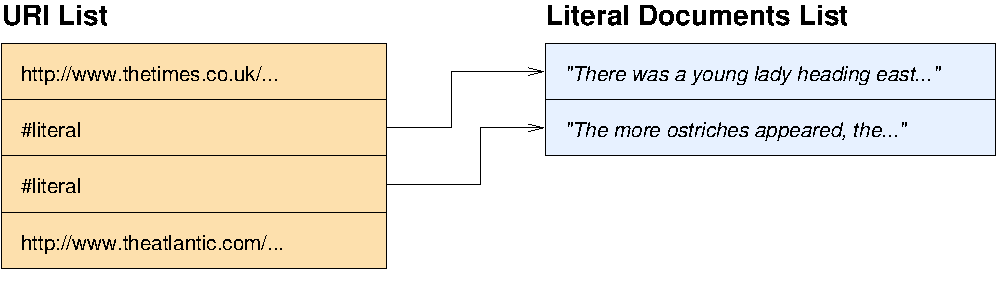
\includegraphics[width=0.8\textwidth]{pictures/twolists}
  \vspace*{-0.4cm}
  \caption{The two lists representing the input documents for an NLP service}  
  \label{fig:twolists}
\end{figure}

Besides the name and the input for a language service, we might need
the client to provide a list of parameters. Therefore, a list of
parameters as described in the previous section is passed along. The
\emph{Value} field of a parameter holds the user-specified value this
parameter should be assigned. Finally, we enable the communication of
user context by passing a representation thereof, as introduced in the
previous section. Table~\ref{tab:invocation} lists all the data
elements transmitted on language service invocation.

\begin{table}
 \centering\small\sffamily
 \begin{tabular}{p{0.22\textwidth}@{\hspace*{4mm}}p{0.45\textwidth}@{\hspace*{4mm}}p{0.2\textwidth}}
   \toprule
   \textbf{Field} & \textbf{Meaning} & \textbf{Example} \\
   \midrule
   NLP service name & The unique identifier of the desired & \emph{English Single} \\
    & language service & \emph{Document Summarizer} \\

    & & \\

   URI list & A list of actual input document URIs and special URIs
   signalling that this document is passed literally. Every input
   document is represented here. & See Fig.~\ref{fig:twolists}  \\

    & & \\

   Document text list & List of document texts, only of those
   documents that are passed literally & See Fig.~\ref{fig:twolists}
   \\

    & & \\

   Parameter list & Transports the parameter values that the client
   specifies & See Table~\ref{tab:param} \\

    & & \\

   User context & The user context, as specified in &
   \emph{[userLangs=en,fr} \\
    & Section~\ref{sec:contextservice} & \emph{docLang=en]}\\
 
   \bottomrule
\end{tabular}
 \caption{Data fields sent from the client when invoking an NLP service}
 \label{tab:invocation}
\end{table}

While language services can most likely be invoked without the current
user context at hand, knowing some facts can prove useful before or
after the invocation. Thus, the invocation could be cancelled if it
is detected that the chosen language service does not fit the input
document(s), or one could tailor the generated output to the user
client's preferences or capabilities.


\subsection{Language Service Results}
\label{sec:response}
Once a language service has finished its work, we want to collect its
results and pass them, in an appropriate format, on to the client. The
\sa architecture allows for different result formats (document
annotation, new documents, results files such as ontologies) and
passes them in a uniform XML response format back to the client.

The basic structure of our response message is rather simple. No
matter what the contents of a message are, they are always be enclosed
in a single \texttt{saResponse} element, the ``sa'' standing for
``Semantic Assistant''. Within this enclosing element, the results
produced by the language service are listed one by one. In
Figure~\ref{list:response1}, this is illustrated for a language
service which produces two different results. Here, they are called
\emph{result1} and \emph{result2}. In reality, they might be an
annotation and a file, or two different annotations, etc.

\begin{figure}[htb]
\begin{lstlisting}[language=XML,xleftmargin=8mm,columns=flexible]
<?xml version="1.0"?>
<saResponse>
    <result1>
        ...
    </result1>
    <result2>
        ...
    </result2>
</saResponse>
\end{lstlisting}
\caption{Schematic structure of an example response with two results}
\label{list:response1}
\end{figure}


\paragraph{Result from GATE Annotations.} With the outer structure of a response
message in place, we have to properly define how specific results are
represented. We take care of annotations first, especially annotations
in GATE (see the GATE documentation for a description of the GATE
document data model if you do not know about document annotations).
Instead of \texttt{result1} or \texttt{result2} in the example above,
we will thus have \texttt{annotation} tags. An important aspect of an
annotation obviously is its name, or type, e.g., \emph{Protein} or
\emph{Person}.  Additionally, for GATE annotations, we include the
annotation set that the annotation is contained in. Thus, we have an
\texttt{annotation} element with \texttt{type} and
\texttt{annotationSet} attributes.

There might be several input document to an NLP service, and an
annotation is always associated with a specific document. Therefore, the
response first lists all input documents within each
\texttt{annotation} tag, using \texttt{document} tags. If the URL of a
document is known, it is included in the corresponding \texttt{document}
tag. However, if a document has been passed literally, we do not have
a URL, so we cannot include it in the response message either. This
seems to be a problem when several documents are passed literally: How
does the client know which result belongs to which document? However,
the order of the documents is maintained as it was when the client
sent them as input.  Therefore, the client is able to correctly assign
the results to the input documents.

For every document, we then list the occurrences of the annotation in
question, using \texttt{annotationInstance} elements. Instances hold a
\texttt{start} and an \texttt{end} attribute, which are character
offsets and which enable the client to locate the instance in the
input text. Moreover, there is a \texttt{content} attribute, which
holds the text located between the \texttt{start} and \texttt{end}
text positions. Finally, annotations can hold an arbitrary number of
so-called features. Features that the system integrator thinks could
be of interest are listed as child elements of the
\texttt{annotationInstance} elements. We can see an example output
with three different annotations (\emph{Date}, \emph{Person}, and
\emph{Location}) and one document in Figure~\ref{list:response2}. The
\emph{Person} and \emph{Location} annotations each have one feature
listed -- \emph{gender} in the case of the person, \emph{locType} in
the case of the location. The document has been passed via URL, which
is why this URL is also included in the response.

\begin{figure}[htb]
\begin{lstlisting}[language=XML,xleftmargin=8mm,columns=flexible]
<?xml version="1.0"?>
<saResponse>
  <annotation type="Date" annotationSet="">
    <document url="http://www.thetimes.co.uk/...">
      <annotationInstance content="yesterday" start="76" end="85">
      </annotationInstance>
      <annotationInstance content="today" start="1056" end="1061">
      </annotationInstance>
      <annotationInstance content="past ten years" start="6477" end="6491">
      </annotationInstance>
    </document>
  </annotation>
  <annotation type="Person" annotationSet="">
    <document url="http://www.thetimes.co.uk/...">
      <annotationInstance content="Tony Blair" start="65"  end="75">
        <feature name="gender" value="male" />
      </annotationInstance>
      <annotationInstance content="Rupert Murdoch" start="2357" end="2371">
        <feature name="gender" value="male" />
      </annotationInstance>
      <annotationInstance content="Mr Blair" start="3133"  end="3141">
        <feature name="gender" value="male" />
      </annotationInstance>
    </document>
  </annotation>
  <annotation type="Location"  annotationSet=""  >
    <document url="http://www.thetimes.co.uk/...">
      <annotationInstance content="Iraq" start="1510" end="1514">
        <feature name="locType" value="country" />
      </annotationInstance>
      <annotationInstance content="Downing Street" start="4576" end="4590">
        <feature name="locType" value="" />
      </annotationInstance>
    </document>
  </annotation>
</saResponse>
\end{lstlisting}
\vspace*{-2mm}
\caption{Result example with three annotations and their detected instances}
\label{list:response2}
\end{figure}


\paragraph{Result Files.} NLP services can also generate new files as
a result -- these can be of any format, depending on the concrete
components deployed in the pipeline. Instead of embedding the file
itself (which can be quite large) directly into the response, we only
pass an identifier for the file, along with some format information.
The client can evaluate this information, and, if it decides to do so,
request the result file itself by using the identifier sent to it. The
server then sends the actual file. Again, we have an example response
in Figure~\ref{list:response3}. The \texttt{outputFile} element holds
format information, both in form of a MIME type string and a human
readable one. The identifier for the result file is given through the
\texttt{url} attribute which refers to the server's file system.

\begin{figure}
\begin{lstlisting}[language=XML,xleftmargin=8mm,columns=flexible]
<?xml version="1.0"?>
<saResponse>
  <outputFile url="file:/tmp/serviceResult-..."
              mimeType="text/html" format="HTML Document" />
</saResponse>
\end{lstlisting}
\vspace*{-2mm}
\caption{Result example with one resulting HTML file}
\label{list:response3}
\end{figure}


\paragraph{Formal Response Message Format Definition.} The complete
response format definition DTD can be found in
Figure~\ref{list:dtd}. It defines documents of the type
\texttt{saResponse}. The \texttt{saResponse} element can contain
arbitrarily many \texttt{annotation} elements and \texttt{outputFile}
elements. Annotations, annotation instances, features, and output
files are defined accordingly.

\begin{figure}
\begin{lstlisting}[language=XML,xleftmargin=8mm,columns=flexible]
<!DOCTYPE saResponse [

  <!ELEMENT saResponse ( annotation*, outputFile* ) >

  <!ELEMENT annotation ( document+ ) >
  <!ATTLIST annotation annotationSet CDATA #IMPLIED >
  <!ATTLIST annotation type NMTOKENS #REQUIRED >

  <!ELEMENT annotationInstance ( feature* ) >
  <!ATTLIST annotationInstance content CDATA   #REQUIRED >
  <!ATTLIST annotationInstance end     NMTOKEN #REQUIRED >
  <!ATTLIST annotationInstance start   NMTOKEN #REQUIRED >

  <!ELEMENT document ( annotationInstance* ) >
  <!ATTLIST document url CDATA #IMPLIED >

  <!ELEMENT feature EMPTY >
  <!ATTLIST feature name  NMTOKEN #REQUIRED >
  <!ATTLIST feature value CDATA   #REQUIRED >

  <!ELEMENT outputFile EMPTY >
  <!ATTLIST outputFile format   CDATA #REQUIRED >
  <!ATTLIST outputFile mimeType CDATA #REQUIRED >
  <!ATTLIST outputFile url      CDATA #REQUIRED >

]>
\end{lstlisting}
\vspace*{-2mm}
\caption{The document type definition (DTD) for our response messages}
\label{list:dtd}
\end{figure}

We have now discussed the most important data exchange processes. In
the next section, we want to ask the question where this data on NLP
services comes from, and how it is organized.

\section{Developing a New Client for the Semantic Assistants Architecture}
We have now covered the most important and interesting implementation
issues, and are ready, with the knowledge we have, to give
step-by-step instructions to connect a client application to our
architecture, and thus to the functionality of NLP services. These
instructions depend a bit on the client implementation language. As we
described earlier, our implementation of the client-side abstraction
layer consists of Java classes packaged in a single Java archive
(\texttt{.jar}) file. Hence, if the client application is able to make
use of Java archives, connecting to our architecture is done as
follows:

\begin{enumerate}
\item Have your application import the Java archive containing the
    implementation of the client-side abstraction layer (CSAL).

\item If necessary, tell the CSAL the address of the Web service
    endpoint. The CSAL classes that need to know the address have a
    default value for it.

\item Create a \texttt{SemanticServiceBrokerService} object, which
    serves as a factory for proxy objects.

\item Create such a proxy object. This is your ``remote control'' to
    the Web service. You can call all methods that have been published
    through the Web service on this object.
\end{enumerate}

After these four steps, a Java-enabled client application can get
lists of available language services as well as invoke these language
services. A code example, where an application obtains such a proxy
object and invokes the \texttt{getAvailableServices} method on it to
find available language analysis services, is shown below:

\begin{lstlisting}[language=Java,xleftmargin=4mm,columns=flexible]
// Create a factory object
SemanticServiceBrokerService service = new SemanticServiceBrokerService();
// Get a proxy object, which locally represents the service endpoint (= port)
SemanticServiceBroker broker = service.getSemanticServiceBrokerPort();
// Proxy object is ready to use. Get a list of available language services.
ServiceInfoForClientArray sia = broker.getAvailableServices();
\end{lstlisting}

A client application developer who cannot use the Java archive that
implements the CSAL still has access to the WSDL description of our
Web services. If there are automatic client code generation tools
available for the programming language of his choice, the developer
can use these to create CSAL-like code, which can then be integrated
into or imported by his application. In this case, the integration
steps would be similar to the steps enumerated above, with the
additional step of generating client-side code from the WSDL
description before the first step.

If there are no such code generation tools, the client application has
to implement the communication with the server itself. To do this, it
must create the SOAP messages that represent method invocations, and
send them to the Web service endpoint. Also, it must receive the
response messages from the server, and extract the relevant
information in them. Usually, however, there are standard libraries
that facilitate these tasks.



% \subsection{Control Flow Overview}
% \begin{figure}[htb]
%   \centering
%   \includegraphics[width=0.5\textwidth]{pictures/seqInvoke1.pdf}
%   \caption{The client invokes a language service and receives a
%     result}
%   \label{fig:seqInvoke1}
% \end{figure}
% Once requested, the language service is executed asynchronously by our
% architecture, allowing the user to continue his work (he can even
% execute additional services).  The sequence diagram in
% Figure~\ref{fig:seqInvoke1} shows the execution of a service
% through the various tiers described in Section~\ref{sec:implementation} Note
% that all low-level details of handling language services, such as
% metadata lookup, parametrization, and result handling, are hidden from
% the client plug-in through our client-side abstraction layer.


\backmatter
\appendix
\bibliographystyle{plainnat}
\bibliography{semassist}

\end{document}




